\documentclass[12pt]{article}

\usepackage{amsmath}
\usepackage{color}
\definecolor{mygreen}{RGB}{28,172,0} % color values Red, Green, Blue
\definecolor{mylilas}{RGB}{170,55,241}
\usepackage{courier}
\usepackage{listings}
\usepackage{graphicx}
\usepackage[a4paper, total={6.5in, 8in}]{geometry}
\usepackage{float}
\usepackage[T1]{fontenc}
\usepackage{xcolor}
\usepackage{titlepic}
\usepackage{caption}
\captionsetup[figure]{labelfont=bf}
\usepackage{textcomp}
\usepackage[nottoc,numbib]{tocbibind}
\usepackage[justification=centering]{caption}
\usepackage{chronosys}

\def\chron@selectmonth#1{\ifcase#1\or Januar\or Februar\or März\or April\or Mai\or Juni\or Juli\or August\or September\or Oktober\or November\or Dezember\fi}

\setlength{\parindent}{0em}
\setlength{\parskip}{1em}
\renewcommand{\baselinestretch}{1.2}

\begin{document}

\pagenumbering{gobble}

\title{\textbf{Object Relational Anomaly Detection for Scene Analysis}\bigbreak
Master Thesis Proposal}
\author{Sashidhar Reddy Kanuboddi}

\maketitle

\titlepic{
\includegraphics[scale = 0.3]{university.jpeg}}

\newpage

\tableofcontents{}

\pagenumbering{arabic}

\newpage

\section{Motivation}

Autonomous mobile robots typically operate in dynamic environments that consist of multiple types of objects. These objects are usually scattered all over the environment. As humans, we have an expectation of where each object should ideally be located, based on our countless observations of similar environments beforehand.

The motivation of this thesis is to enable robots to have a similar understanding of its surroundings. The objective is to implement a learning framework that uses annotated 3D point clouds of different configurations of a particular type of scene, say a living room or an office, and extracts features relevant to the positional and angular bearings of each object with respect to other objects, and finally, is able to identify anomalies when presented with new unseen instances of the scene based on what it has learnt from all the training instances.



\section{Modeling Spatial Relations of Objects in a Scene}

This thesis will essentially implement a framework from STRANDS, a collaborative European research project \cite{STRANDS}. The steps to implement the framework are as follows:

\begin{enumerate}
\item{Collecting a dataset of point clouds, consisting of different configurations of a particular type of scene.}
\item{Manually annotating each point cloud with 3D bounding boxes placed over each object.}
\item{Extracting features from this annotated point cloud dataset, such as pose and angular bearing of each object w.r.t a fixed frame of reference and w.r.t other objects, volume of each object etc.}
\item{Fitting a model over the extracted features, eg. a Gaussian Mixture Model.}
\item{Using the fitted model to compute scene similarity score for new scenes. Scenes with a score below a certain threshold would be declared anomalous.}
\end{enumerate}




\section{Thesis}

Each of the above mentioned steps is described in more detail below:

\subsection{Dataset of Point Clouds}

High resolution point clouds of a scene with different configurations shall be collected. The idea, at the moment, is to capture the point cloud of a bookshelf filled with objects in order to learn about the underlying structure of which objects go on which shelf. By different configurations, it is meant that the bookshelf will not always contain the same objects, but much like a bookshelf in a house, it can contain different objects at different times, and sometimes the same object maybe on different shelves.

Capturing the point clouds is not a trivial task, as we need high resolution point clouds of the entire scene, which means scanning with a 3D sensor (Microsoft Kinect, Asus Xtion) over multiple passes and fusing the point cloud from each pass to form one dense high resolution point cloud. A software called KinectFusion from Microsoft Research\cite{KinectFusion} claims to accomplish this task in real time with the help of heavy graphics hardware and it is proposed to use this tool in this thesis.


\begin{figure} [H]
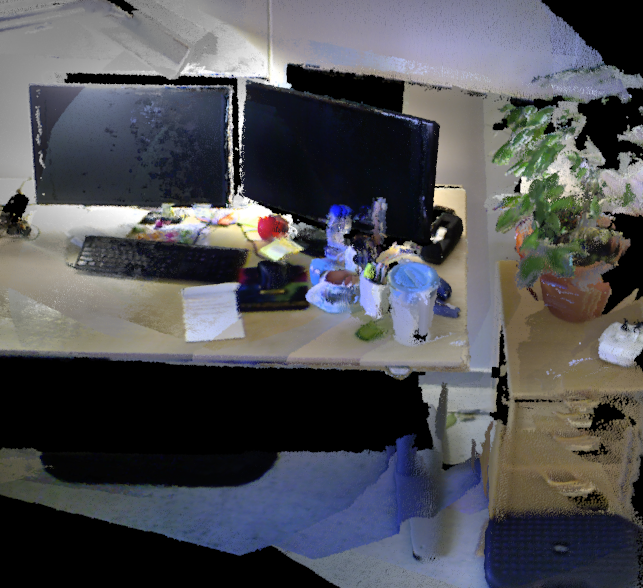
\includegraphics[scale = 0.30]{pcl.png}
\centering
\caption{\textbf{High Resolution Point Cloud of an Office Desk \cite{KTH Dataset}}} 
\end{figure}


\subsection{Manual Annotation of the Dataset}

Once the point clouds have been gathered, each of them will be manually annotated by using a tool developed by KTH Sweden for their research. This tool allows us to graphically put 3D bounding boxes over each object in the scene and export information about the pose (w.r.t a fixed frame of reference) and dimensions of each bounding box to an XML file.

\begin{figure} [H]
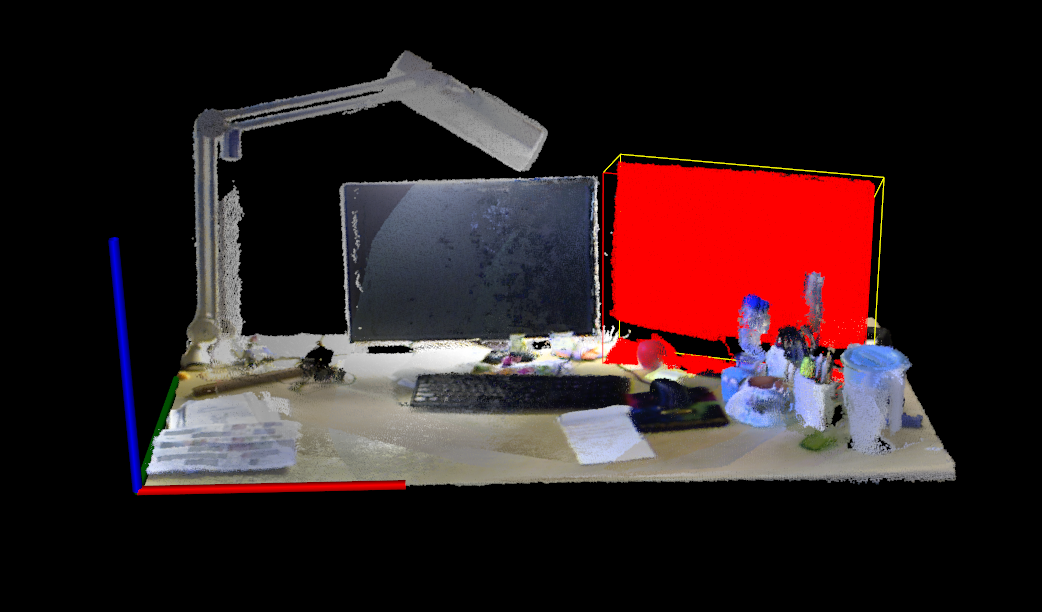
\includegraphics[scale = 0.30]{pcl_annotated.png}
\centering
\caption{\textbf{Annotated Point Cloud with Bounding Box over a Monitor \cite{KTH Dataset}}} 
\end{figure}

\subsection{Extraction of Features}

Using the information in the XML files obtained from the point cloud annotation tool, the following features shall be extracted \cite{STRANDS}:

\paragraph{Single Object Features ($f_{o_i}$)}

\begin{itemize}
\item{3D position of the object centroid}
\item{2D (horizontal) bearing of object centroid from the origin}
\item{Volume of the object}
\end{itemize}

\paragraph{Object Pair Features ($f_{o_i, o_j}$)}

\begin{itemize}
\item{d($C_{o_i}$, $C_{o_j}$), where d is the Euclidean distance and $C_{o_i}$, $C_{o_j}$ are the centroids of objects $o_i$ and $o_j$ respectively}
\item{Ratio of the object volumes}
\item{$d_z$($C_{o_i}$, $C_{o_j}$), where $d_z$ if the vertical displacement between the two objects}
\end{itemize}


The possibility of adding more features which can improve the model shall also be explored in this thesis.

\begin{figure} [H]
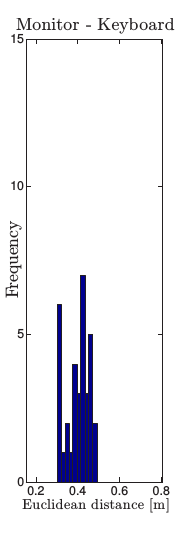
\includegraphics[scale = 0.50]{histogram.png}
\centering
\caption{\textbf{Histogram of one of the features, the Euclidean Distance between two objects \cite{KTH Dataset}}}
\end{figure}


\subsection{Fitting a Model}

A Gaussian Mixture Model (GMM) shall be used to model the aforementioned features.

\paragraph{Object class Modeling}

To model the object class category, we fit a GMM over each set of single object features collected from all the scenes:

\[
GMM(f_{o_i}, \mu_{o_i}^z, \Sigma_{o_i}^z) = \sum_{z=1}^{n_c} \pi_z \frac{1}{K}
exp(-\frac{1}{2} \zeta_{o_i}^z)
\]
where: 
\[\zeta_{o_i}^z = (f_{o_i} - \mu_{o_i}^z)^T \Sigma_{o_i}^{z - 1} (f_{o_i} - \mu_{o_i}^z)) \]
\[K = \sqrt{(2\pi)^{dim}|\Sigma_{o_i}^z|} \text{   ,   } 
\pi_z \geq 0 \text{   ,   }
\sum_{z = 1}^{d}\pi_z = 1\]
$n_c$ is the number of mixtures, $\pi_z$ is the weight of the $z^{th}$ mixture, $\mu_{o_i}^z$ is the mean of the normal distribution, $\Sigma_{o_i}^z$ is the covariance matrix and $dim$ is the dimensionality of the feature space. 

\paragraph{Learning object pair relationships}

To learn these relationships, we fit a GMM again over each set of object pair features collected from all the scenes.


\subsection{Computation of Scene Similarity Score}

Once the model is trained on multiple instances of a scene type, a new instance is given to the program and the question now becomes: how similar is this new instance to our set of trained scenes? Is there something wrong with this new instance? 

For computing the scene similarity score, we extract the feature vectors from the new instance and use the fitted model to compute the probability of these features belonging to the same distribution and hence, the same type of scene. 

Ideally, for implementation on a real robot, the feature extraction from the new instance step should be performed automatically with the help of a perception software that is able to place 3D bounding boxes around objects, but that is outside the focus of this thesis, hence the new instance shall have a manually annotated point cloud as well.

Using the learned models, the scene similarity score is predicted as follows:

\[sim(s_u, S_t) = \sum_{o_i, o_j \in s_u} P(f_{o_i, o_j}|S_t)P(o_i, o_j) + 
\sum_{o_i \in s_u} P(f_{o_i}|S_t)P(o_i)\]
where $sim(s_u, S_t)$ is the scene similarity score of a new unknown instance $s_u$ with respect to the modeled scene class type $t$, $S_t$ and $f_{o_i}$, $f_{o_i, o_j}$ are feature vectors from the new instance. 

A threshold shall be fixed empirically after running the algorithm through some known anomalous scenes and this threshold shall then be used to detect future anomalous scenes.

Furthermore, to identify the source of the anomaly in the scene, having thresholds for individual terms in the summation shall also be explored.


\section{Timeline}

\begin{figure} [H]
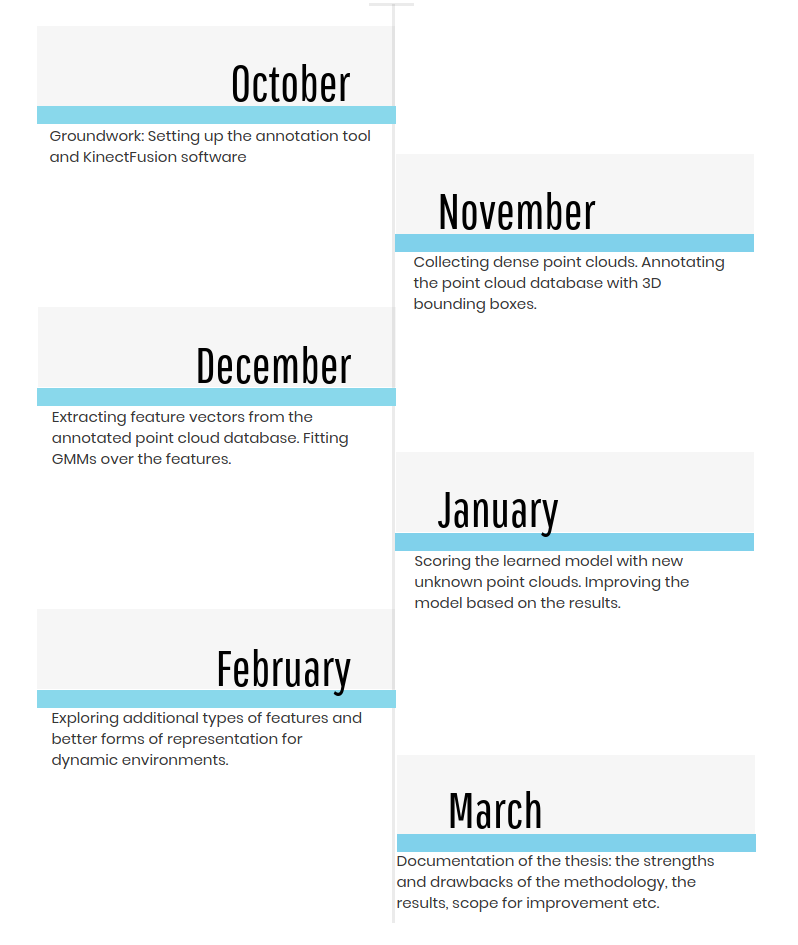
\includegraphics[scale = 0.60]{timeline3.png}
\centering

\end{figure}

%\newpage
%
%\section{References}
%
%\begin{enumerate}
%\item{M. Alberti, J. Folkesson and P. Jensfelt. Relational Approaches for Joint Object Classification and Scene Similarity Measurement in Indoor Environments. \textit{AAAI Spring Symposium,} 2014}
%\item{R. Newcombe, et al. KinectFusion: Real-Time Dense Surface Mapping and Tracking. \textit{ISMAR,} 2011}
%\end{enumerate}


\newpage

\begin{thebibliography}{9}

\bibitem{STRANDS} 
M. Alberti, J. Folkesson and P. Jensfelt. 
\textit{Relational Approaches for Joint Object Classification and Scene Similarity Measurement in Indoor Environments}. 
AAAI Spring Symposium, 2014.
 
\bibitem{KinectFusion} 
R. Newcombe, et al. 
\textit{KinectFusion: Real-Time Dense Surface Mapping and Tracking}. 
ISMAR, 2011.

\bibitem{KTH Dataset} 
A. Thippur, et al. 
\textit{KTH-3D-TOTAL: A 3D Datset for Discovering Spatial Structures for Long-Term Autonomous Learning}. 
ICARCV, 2014.
 
\end{thebibliography}

\end{document}










